\documentclass[sigconf]{acmart}
\usepackage{amsmath}
\usepackage[utf8]{inputenc}
\usepackage{color,soul}
\usepackage{tikz}
\usetikzlibrary{shapes.geometric, arrows, bayesnet, calc, positioning}
\usepackage{tikz}
\usepackage{pgfplots}
\usepackage{pgf}
\usetikzlibrary{calc}
\usetikzlibrary{positioning}
\usetikzlibrary{angles,quotes}
\usetikzlibrary{backgrounds}
\usetikzlibrary{fit}
\usetikzlibrary{arrows}
\usetikzlibrary{arrows.meta}
\usetikzlibrary{shapes.symbols}
\usetikzlibrary{shadings}
\usetikzlibrary{shapes}
\usetikzlibrary{fadings}
\usetikzlibrary{bayesnet}
\usetikzlibrary{matrix}
\usetikzlibrary{plotmarks}
\usetikzlibrary{intersections}
\usetikzlibrary{pgfplots.fillbetween}
\pgfplotsset{compat=1.14}
\usepackage{colortbl}
\usetikzlibrary{shapes,decorations,arrows,calc,arrows.meta,fit,positioning}
\tikzset{
	-Latex,auto,node distance =1 cm and 1 cm,semithick,
	state/.style ={ellipse, draw, minimum width = 0.7 cm},
	point/.style = {circle, draw, inner sep=0.04cm,fill,node contents={}},
	bidirected/.style={Latex-Latex,dashed},
	el/.style = {inner sep=2pt, align=left, sloped}
}

\begin{document}

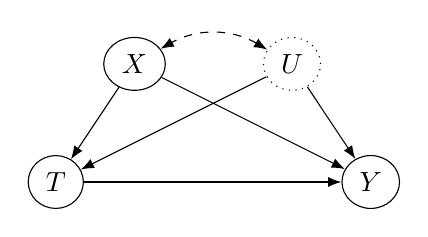
\begin{tikzpicture}
\centering
    % x node set with absolute coordinates
    \node[state] (t) at (-2,0) {${T}$};
    \node[state] (y) at (2,0) {${Y}$};

    \node[state,dotted] (z) at (1,1.5) {${U}$};

    \node[state] (x) at (-1,1.5) {$X$}; 

    % Directed edge
    \path (x) edge (t);
    \path (x) edge (y);
    \path (t) edge (y);
    
    \path (z) edge (y);

    \path (z) edge (t);
    
    % Bidirected edge
    \path[bidirected] (z) edge[bend right=30] (x);
\end{tikzpicture}

\end{document}